%- block legend
Douglas está muito preocupado com um grande vazamento de senhas de sua rede
social favorita. Por isso, ele
decidiu que irá escolher uma nova senha para sua rede.
Metódico que é, Douglas decidiu que irá escolher sua nova senha usando seu
\textit{disco de senha}, que é um disco circular contendo $N$ letras minúsculas.
A senha será escolhida da seguinte forma:
\begin{enumerate}
    \item Douglas irá escolher alguma letra no disco para ser a primeira letra
    da senha;
    \item A senha será formada percorrendo o disco em sentido horário, a partir
    da primeira letra, concatenando as letras percorridas;
    \item A senha deverá ter no mínimo 1 e no máximo $K$ letras.
\end{enumerate}

Quantas senhas \textit{distintas} podem ser formadas dessa maneira?

%- endblock

%- block input
A primeira linha contém dois inteiros $N$ e $K$ ($1 \leq K \leq N \leq
        \VAR{vars.N.max | sci}$), o número de letras no disco e o tamanho máximo
da senha, respectivamente.
A segunda linha contém $N$ letras minúsculas indicando as letras no disco, em
sentido horário, a partir de qualquer uma delas.
%- endblock

%- block output
Imprima uma linha com o número de senhas distintas que podem ser formadas.
%- endblock

%- block notes
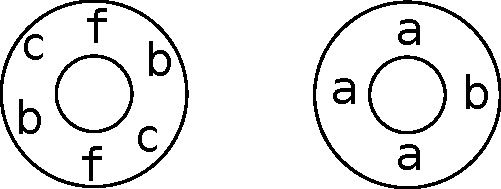
\includegraphics[scale=0.6]{disco0.pdf}\\
Os discos acima representam os dois primeiros exemplos de entrada.
No primeiro exemplo, as senhas que podem ser formadas com até $K=3$ letras são
\texttt{b}, \texttt{c}, \texttt{f}, \texttt{bc}, \texttt{cf}, \texttt{fb},
\texttt{bcf}, \texttt{cfb} e \texttt{fbc}, totalizando 9 senhas distintas.
No segundo exemplo, as senhas que podem ser formadas com até $K=2$ letras são
\texttt{a}, \texttt{b}, \texttt{aa}, \texttt{ab} e \texttt{ba}, totalizando 5 senhas distintas.

%- endblock

%- block editorial
This is the editorial.
%- endblock
